
%%%%%%%%%%%%%%%%%%%%%%% file typeinst.tex %%%%%%%%%%%%%%%%%%%%%%%%%
%
% This is the LaTeX source for the instructions to authors using
% the LaTeX document class 'llncs.cls' for contributions to
% the Lecture Notes in Computer Sciences series.
% http://www.springer.com/lncs       Springer Heidelberg 2006/05/04
%
% It may be used as a template for your own input - copy it
% to a new file with a new name and use it as the basis
% for your article.
%
% NB: the document class 'llncs' has its own and detailed documentation, see
% ftp://ftp.springer.de/data/pubftp/pub/tex/latex/llncs/latex2e/llncsdoc.pdf
%
%%%%%%%%%%%%%%%%%%%%%%%%%%%%%%%%%%%%%%%%%%%%%%%%%%%%%%%%%%%%%%%%%%%


\documentclass[runningheads,a4paper]{llncs}

\usepackage{amssymb}
\setcounter{tocdepth}{3}
\usepackage{graphicx}
\usepackage[T1]{fontenc}
\usepackage[utf8]{inputenc}
\usepackage[italian]{babel}

\usepackage{url}
\urldef{\mailsa}\path|{alfred.hofmann, ursula.barth, ingrid.haas, frank.holzwarth,|
\urldef{\mailsb}\path|anna.kramer, leonie.kunz, christine.reiss, nicole.sator,|
\urldef{\mailsc}\path|erika.siebert-cole, peter.strasser, lncs}@springer.com|    
\newcommand{\keywords}[1]{\par\addvspace\baselineskip
\noindent\keywordname\enspace\ignorespaces#1}

\begin{document}

\mainmatter  % start of an individual contribution

% first the title is needed
\title{On the liability of TOR Exit Relay operators}

% a short form should be given in case it is too long for the running head
\titlerunning{}

% the name(s) of the author(s) follow(s) next
%
% NB: Chinese authors should write their first names(s) in front of
% their surnames. This ensures that the names appear correctly in
% the running heads and the author index.
%
\author{Alessio Trivisonno}
%
\authorrunning{}
% (feature abused for this document to repeat the title also on left hand pages)

% the affiliations are given next; don't give your e-mail address
% unless you accept that it will be published
\institute{University of Trento}

%
% NB: a more complex sample for affiliations and the mapping to the
% corresponding authors can be found in the file "llncs.dem"
% (search for the string "\mainmatter" where a contribution starts).
% "llncs.dem" accompanies the document class "llncs.cls".
%

\toctitle{}
\tocauthor{}
\maketitle


\begin{abstract}
The abstract should summarize the contents of the paper and should
contain at least 70 and at most 150 words. It should be written using the
\emph{abstract} environment.
\keywords{Tor, Exit Node, Operator, ISP, Internet Service Provider, Liability}
\end{abstract}


\section{Introduction}

\section{Background}

\subsection{What is TOR}

Tor is a free and open source software aimed to enable anonymous communication on the web. It is the most used and secure \textit{Privacy Enhancing Technology} that is available now. Tor belongs to the same class as VPNs, Proxies and DNS Bypass. However it is the only technique that has been proved truly ensure your anonymity on the web. For this reason Tor has become more and more popular during these years, especially in countries where censorship is most suffered. Like China and Saudi Arabia.Today Tor is used on average by 2 Million users every day.

The name Tor stands for ``The Onion Router`` 
which is the technology at the core of this software.The Onion Routing is a networking mechanism that ensures encryption and 
anonymity in a communication between two endpoints. Such endpoints might be two users (in a P2P communication) or a user and a web service (like a website). The connection between 
endpoints is routed along an encrypted channel that jumps all over the world inside the Tor Network. Each relay has the knowledge of only the previous and the 
following nodes in the chain of jumps and this makes the complete picture of the communication hidden from anyone.\footnote{Although the technology is very strong and secure there are still many attacks that can undermine the anonymity of the Tor users} \cite{CCDCOF}


\subsection{How It Works}
Tor achieves such anonymity with a very simple architecture that relies on cryptography.
It is composed of basically three entities: 
\begin{itemize}
    \setlength\itemsep{0.7em}
    \item The Directory Servers
    \item Middle Relays
    \item Exit Relays
\end{itemize}
The Directory Servers advertise the entry points of the Tor Network to the client.
The network itself is made of components called Relays. Those are of two different types: one is called Middle Relay and another one Exit Relay.
Tor creates a circuit starting from the end user to the destination that jumps on 
different hops (Relays) during its path. At each jump the intermediate packet is encapsulated into an additional layer of encryption, achieving the fact that each node knows only its previous and following hop. From the moment that the request of the end user 
enters the network it jumps randomly on a set of Middle Relays before reaching the Exit Relays. 
Those are the points in which the request of the end user makes the last step towards 
the final destination. See Fig \ref{fig:fig_tor_arch}



Another fundamental function of Tor are the so called Hidden Services. A Hidden Service is used to keep the physical location of a server anonymous and uses a mechanism called rendezvous. The client's request and the server's response meet in a designated random point in the Tor Network. In this way the anonymity is preserved from both the user and the server side. See Fig \ref{fig:fig_tor_hid}
\begin{figure}[]
    \center{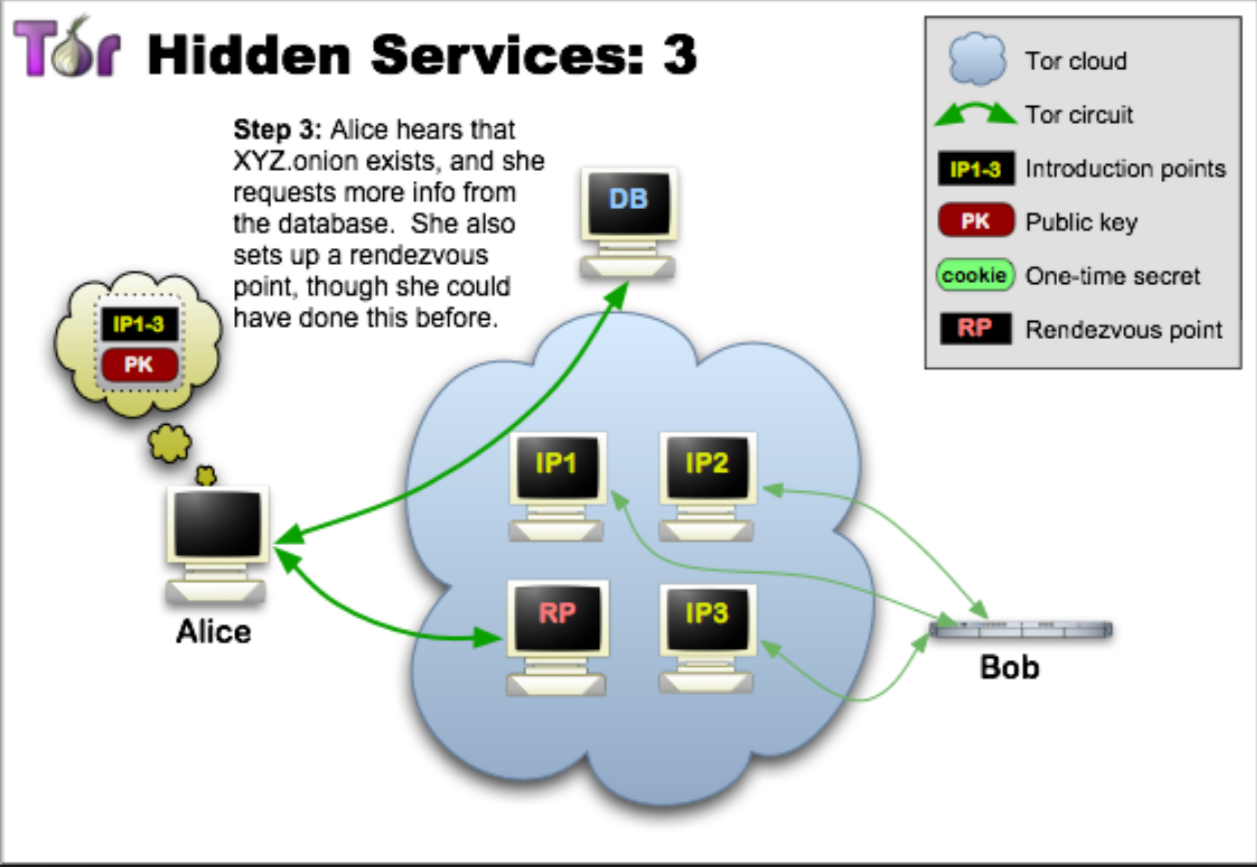
\includegraphics[width=0.5\textwidth]
        {./figures/tor_hidden.png}}
        \caption{ Tor Hidden Service Architecture}
        \label{fig:fig_tor_hid}
\end{figure}

\begin{figure}[]
    \center{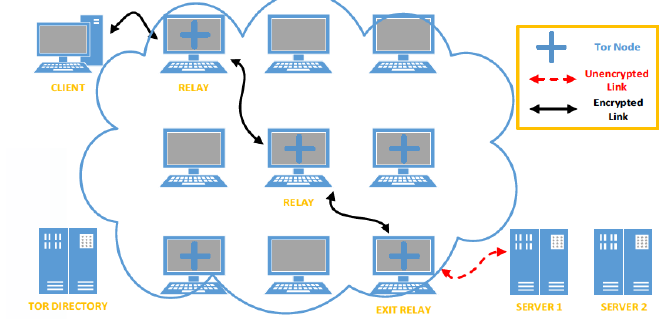
\includegraphics[width=0.5\textwidth]
        {./figures/tor_arch.png}}
        \caption{ Tor architecture}
        \label{fig:fig_tor_arch}
\end{figure}


The technology relies solely on the efforts of volunteers (individuals or organizations) all over the world who run the relays and provide the access to the internet using their own internet access point.



\section{For what Tor is used for}
Tor has been developed with the idea that anyone should be able to surf the internet and express their belief without being monitored by others, not even governments. Among its main usage we can find privacy protection for individual unwilling to give away their navigation data to ISPs. In the business filed Tor is used to ensure confidentiality and for conducting  research on competitors without leaving traces. Similarly Tor can be used for intelligence gathering by government's body like the U.S. Navy, in fact they where the ones who  developed this very idea of the Onion Routing. It can also be used to protect the identity of sources for journalists, like whistle-blowers. And It can also help activists to report abuse or organize meetings, as it happened during the Egyptian Revolution of 2011. \cite{WASH_715}

\begin{figure}[]
    \center{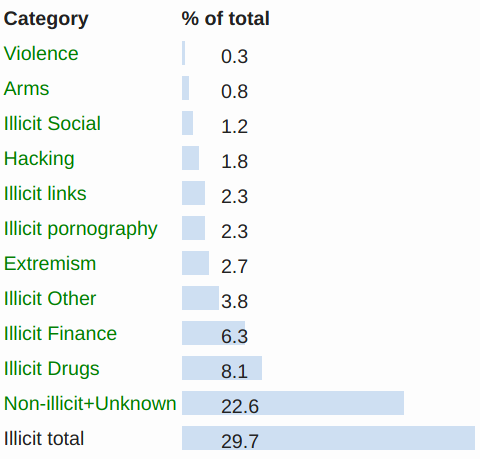
\includegraphics[width=0.5\textwidth]
        {./figures/tor_illicit.png}}
        \caption{Web-Based Onion Services in February 2016 (Source Wikipedia.org)}
        \label{fig:fig_tor_ill}
\end{figure}

Beside that good things, Tor has been accused to be a safe harbor for criminal activity, especially regarding child pornography and drug dealing. As shown in figure \ref{fig:fig_tor_ill} the amount of illicit activity percentage on the overall onion services is high (almost 30\%). For example famous were the cases of the sites PlayPen
\footnote{}
and  the PlayPen investigation the American National Security Agency identified thousands of computers around the globe that used Tor to visit the Playpen site. This led to court 137 American citizens for possession of video depicting images with child pornography.SilkRoDuringad that led to the incarceration of many users and maintainer of those sites. 

\section{The problem: Liability of Tor Exit Relays Operators}
Since the Tor Exit Relay Operators are the one that carry on the \textit{last mile communication} they are the one that are most exposed in terms of legal actions.
As shown in Fig \ref{fig:fig_tor_arch} the connection between client to relay and relay to relay is encrypted
and does not cause any problems to the Middle Relay operator. The Exit Relays instead, are the most exposed part of the network, since the communication between
the client and the server is at this stage unencrypted, making the request look like as it is the 
Exit Relay which is originating that traffic. 
In fact, from the technological prospective, if from their server transit a request from a generic Tor user for a site that hosts illicit content, such request cannot be distinguished from the normal traffic of the person who is operating the Exit Relay. 
Exit Relays behave in the same way as normal relay does, they remove the source IP address of any incoming internet packet, and replaces it with its own IP address as a source, lastly it forwards the request to the next hop. But what is different from the other relays is that in this case the last hop is the final destination and as shown in Fig. \ref{fig:fig_tor_arch} the communication between the Exit Relay and the destination server is no longer secured by the Tor protocol \footnote{The communication can still be encrypted at application level with HTTPS but the source and destination IP address are no longer anonymised}. 

There is not much research in the field of liability of Tor operators and people have tried over the years to relate the activity of such people to the activity of the Internet Service Providers. But can Tor Operators be considered as ISP?
As it was explained in the section 2 the activity of such people is just to forward internet packets from one node to another. Middle Relays can by no means know nor the content of the packet nor the destination, 
\footnote{Because they know just the precious and the following hop}
which makes any surveillance  of the traffic technologically impossible. Exit relays insted do know the final destination of the user request and have the technological power to do at list controls to enact cencorship. However as we will see in the following section their activity, because of the way they handle the data, falls in the "mere conduit" safe harbor, which shields them from anu liability. 
TODO: Company Terms of Service, like Aruba

\section{The case Austrian Regional Crime Court vs William Weber}
In this section I will present the case of Austrian regional criminal court in Graz vs. W. Weber. This case sees W.Weber, a tor exit node operator being sentenced by the court for aiding the distribution of child pornography. I will discuss the case and talk about the reason why he was held accountable and what where the court motivation for that.

On June 30th 2014 William Weber a Tor Exit Node Operator was sentenced to 3 months of jail and 3 years of probation for helping the distribution of child pornography on through his server.

As we discussed in the previous paragraph, Tor Exit Node Operators are the one that are most exposed in terms of criminal liability since they supply their internet access point and their unique IP address to the Tor community.

The main reason why the court judged W.Weber liable of aiding the distribution of child pornography was that he was intercepted while talking to an anonymous person on the web about the possibility of hosting child pornography on his server. He said: 
\begin{quote}
    \textit{ "You can host 20TB child porn with us on some encrypted HDD”[...] “You can host child porn on our servers” [...] “If you want to host child porn ... I would use Tor.”}
\end{quote}
That showed to the Court that not only was he at least aware that his Tor node could have been used to do distribute child pornography, but also he does not disapprove that.
However he declared on his blog that this conversation was used out of context and that he was just talking hypothetically. 
Despite that, he was found guilty because (as stated by Huťko \cite{HUSOVEC}):
\begin{quote}
\textit{
    The Austrian Court found that this activity may lead to criminal liability for aiding and abetting of a crime of distribution of child pornography when coupled with other circumstances.}
\end{quote}
The other circumstances that invalidated the \textit{mere conduit} safe harbour were these very transcript. In fact as stated by Art.12 of the eCommerce Directive 
\begin{quote}
    \textit{1. Where an information society service is provided that consists of the transmission in a communication network of information provided by a recipient of the service, or the provision of access to a communication network, Member States shall ensure that the service provider is not liable for the information transmitted, on condition that the provider:\\
(a) does not initiate the transmission;\\
(b) does not select the receiver of the transmission; and\\
(c) does not select or modify the information contained in the transmission.}
\end{quote}

Also it is to say that forensic experts have reconstructed some images depicting pornographic acts of children. However he could not be found guilty since there was no evidence that these picture were effectively downloaded by him or by the the automatic caching mechanism. And he was by far protected by the article 12 section 2 of the eCommerce Directive for these evidence:

\begin{quote}
    \textit{2. The acts of transmission and of provision of access referred to in paragraph 1 include the automatic, intermediate and transient storage of the information transmitted in so far as this takes place for the sole purpose of carrying out the transmission in the communication network, and provided that the information is not stored for any period longer than is reasonably necessary for the transmission.}
\end{quote}

But, since he was intercepted having that conversation with the anonymous user, he was actively collaborating with the intent of doing illegal activities with that person. That invalidated the liability exemption from "mere conduit" considering the Recital 44 of the Directive:

\begin{quote}
    \textit{
(44) A service provider who deliberately collaborates with one of the recipients of his service in order to undertake illegal acts goes beyond the activities of "mere conduit" or "caching" and as a result cannot benefit from the liability exemptions established for these activities.}
\end{quote}

At the end of this first litigation he decided to do not go in further trials and accept the sentence.

This decision demonstrates that Tor Exit Node Operators should be very cautious when operating their activity not only from the technology prospective, but also from the legal one. However as cited in \cite{HUSOVEC} \textit{we should be really careful in keeping the standard of "deliberate collaboration" very high, otherwise it might be easy to criminalize Tor Exit Nodes operators}. . Criminalizing the Tor operators would be very easy in countries \textit{with less legitimate criminal offences such as anti-state propaganda crimes} \cite{HUSOVEC}. Without their valuable work the whole anonymity network phenomena would not exist. They in fact operate in one of the most crucial point of the architecture, they connect the anonymous world with the real world, without that connection the anonymity world has no point to exist.

However this sentence has not to be considered as a sentence against Tor. Tor is still perceived as an important tool to ensure privacy and secrecy, as stated by  Shubert in the Constitutional Court who said that \textit{"privacy and especially the secrecy of communication on the Internet have to be protected"} and that the legality of Tor should not be challenged. \cite{PCW}

\section{The situation in Italy} 
In this section I will present how in Italy is handled the liability of ISP illustrating some examples on court decision, as the sentence n. 54946/2016 of the Corte di Cassazione. And also I will discuss the d.lgs 70/2003, with particular interest to art 14, art 15 and art 16.

In Italy rules the Art 2043 of the Civil Code which says \textit{"Whatever malicious or negligent misconduct, or negligence, which causes an unfair damage to another person, obliges who committed the fact to pay the compensation"}. 

In the 2003 the European Directive commonly known as eCommerce regulation was introduced in the corpus of the law with the D.L. 70 of 2003 \textbf{SISTEMA}!!
\footnote{Decreto legislativo 9 aprile 2003, n. 70 Attuazione della direttiva 2000/31/CE relativa a taluni aspetti giuridici dei servizi della società dell'informazione, in particolare il commercio elettronico, nel
mercato interno; pubblicato in G. U. n. 61 del 14.04.2003.
}
\subsection{The case Google vs Vivi Down}
\subsubsection{The facts}
Vivi Down is an association that aims to aid people affected by autism.\\ 
Google Video is an online platform where registered users can upload their videos and share them among the community. \\ 
On May 2006 some highschool students from Turin uploaded on the platform Google Video a video depicting them in the act of insulting and hitting a boy affected by autism. Furthermore the bullies said to be part of the association Vivi Down. After 2 months the video gained a lot of success for the time, scoring more than 5000 views before it was taken down by Google. 
Vivi Down sued not only the boys who commit the crime but also Google bringing as support the art 40 of the Italian Criminal Code.
The accuses that Vivi Down addressed to Google were defamation and privacy infringement, because of the disclosure of the extremely personal data about the health of the autistic boy in the video.
\footnote{"Non impedire un evento, che si ha l'obbligo giuridico di impedire equivale a cagionarlo" - Art 40 of the Italian Criminal Code}
\subsubsection{The first level ruling}
The trial was carried out by the public prosecutor's office of Milan, being Milan the legal residence of Google Italy\cite{NOTARI}. 
In 2010 the Court found the Google managers not guilty of the accuses of defamation since the activity of Google and his platform Google Video falls into the shield of the European eCommerce regulation 2000/31/CE. In particular they applied the concept discussed above regarding the \textit{mere conduit safe harbor} for which Google Video act as a simple hosting service and for this is not responsible for any illegal acts performed by his users, until he became aware of such infringement.
But the Court also said that although the 2000/31/CE forbids the obligation of surveillance of the content that people upload on a service provider's platform
In particular they applied the recital 47 which says \footnote{
\textit{
 Member States are prevented from imposing a monitoring obligation on service providers only with respect to obligations of a general nature; [...]}
 },
they should have informed in a clean and explicit way the boys who uploaded the video on the requirement of collecting the explicit consent of the autistic boy  for the disclosure of such private information. They correlated this to the Art 13 of the Italian Privacy Code. \footnote{\textit{The interested party, or the person whose personal data has been collected, is informed beforehand either orally or in writing}}

Furthermore the Court pointed out that there might have been a malicious intent in the act of Google of sharing the video containing such information because they turned a profit through the platform Google AdWord. 
\footnote{AdWord is a service given by Google to target user with personalized advertisement based on their browser history} 
And since the platform AdWord was able to track the users behaviour and suggest video raccomandation the Court changed the scope of Google Video from Hosting to Content Provider, which does not benefit from the exemption of the 2000/31/CE. 
\footnote{
Cfr. M. De Cata, \textit{La responsabilità civile dell'Internet service provider, Milano, 2010, pp. 70-71}, he defines the host provider as someones who gives some memory space of his server for the hosting of a web service, whereas the content provider is someone who gives on its own content to the public as has therefore more responsibility on the content he delivers. 
}.

\subsubsection{The Second level ruling}
The case was then appealed to the Corte D'Appello of Milan
\footnote{
Corte d’Appello di Milano, I sezione penale, sentenza n. 8611/12, 21 dicembre 2012.
} where the Court, respectful the Privacy Code violation of the article 13, ruled that the Google Managers were not guilty since the art 167 says that the violation occurs only if the author acted not conforming the regulation. And that none of the part of this article force the ISP to educate the user concerning the content of the Privacy Code. \cite{NOTARI}
They also refused the ruling of the first level ruling about the malicious intent of Google in sharing the video with the justification that there were no specific links pointing to the video. Furthermore the Court stated the non-involvement of Google as they acted as only a hosting refusing the scope change in Content Provider and gave all the responsibility of the illegal act to the "uploaders". 

\subsubsection{The Third level ruling}
The case was finally brought to the Corte di Cassazione who ultimately absolved Google confirming their non-involvement with respect to the European eCommerce Directive 2000/31/CE. As confirmation of non-involvement in the illicit activity was brought as an exaple the fact that Google immediately removed the video from his platform once they became aware of the privacy violation from the authorities. Thus Google acted in full compliance with the recital 46 of the 2000/31/CE \begin{quote}
    \textit{
    In order to benefit from a limitation of liability, the provider of an information society service, consisting of the storage of information, upon obtaining actual knowledge or awareness of illegal activities has to act expeditiously to remove or to disable access to the information concerned; 
    }
\end{quote}



\section{Conclusion and Future Work}

From the research that has been conducted it was seen that besides the case at section 4 there were no legal actions against Tor Exit Relays operators. Maybe because they generate kind of traffic that is highly recognisable and that makes clear the non-involvement of the operators in the content of the communication.
Even the NSA has demonstrated no interest in prosecuting the exit operators, aiming instead to the users as it was done with the PlayPen case. Also it is to say that the majority of sites that host illicit activity, if not all of them, use the technology of Hidden Services which makes the detection of the illicit activity even harder to investigate.


\newpage


\begin{thebibliography}{9}

\bibitem{CCDCOF}
Emin \c{C}alı\c{s}kan, Tom\'{a}\u{s} Min\'{a}rik, Anna-Maria Osula (2015).
\textit{Technical and Legal Overview of the 
Tor Anonymity Network}.\\
NATO Cooperative Cyber Defence Center of 
Excellence, Tallin, Estonia

\bibitem{WASH_715}
    Keith D. Watson. (2012)
    \textit{ THE TOR NETWORK: A GLOBAL INQUIRY INTO THE LEGAL STATUS OF ANONYMITY NETWORKS . }
    Washington University Global Studies Law Review

\bibitem{EFF_PLAYPEN}
    Electronic Frontier Foundation\\
    \textit{The Playpen Cases: Frequently Asked Questions}
    link: https://www.eff.org/it/pages/playpen-cases-frequently-asked-questions\\
    date of last visit: "03/04/2019"
    
    \bibitem{HUSOVEC}
    Huťko´s Technology Law Blog\\
    \textit{Austrian Court Sentenced a Tor Exit Node Operator}
    link:     http://www.husovec.eu/2014/07/austrian-court-sentenced-tor-exit-node.html
    date of last visit: "12/04/2019"
    
    \bibitem{PCW}
    Loek Essers, PC WORLD\\
    \textit{Tor exit node operator convicted of abetting spread of child porn}
    link:         https://www.pcworld.com/article/2452320/tor-exit-node-operator-convicted-of-abetting-spread-of-child-porn.html
    date of last visit: "12/04/2019
    
     \bibitem{NOTARI}
    Federica Notari, Amministrazione In Cammino\\
    \textit{    La controversa responsabilità dell’Internet Service Provider in materia di privacy nella giurisprudenza europea e interna: il caso Google}



\end{thebibliography}


\end{document}